\appendix

\section*{Backup}

\begin{frame}[noframenumbering,plain]
    \vfill
    \begin{center}
        {\Huge\bfseries Backup slides}\\[1em]
        {\large Reachability, proofs, postulates, performance, scenarios}
    \end{center}
    \vfill
\end{frame}

%========================================================================
% Limitations of a propositional encoding (Thesis \S4.2)
%========================================================================

\begin{frame}[noframenumbering]{Backup, a propositional encoding of the drill chain works\dots}
    \hypertarget{bk:naive-drill}{}
    To build a propositional encoding from a planning problem, use the following rules:
    \begin{itemize}
        \item Each goal becomes a fact
        \item Each produced proposition implies its operator's preconditions and the negation of its delete effects
        \item The closed-world assumption negates every proposition that no operator produces and that is absent from $I$
    \end{itemize}

    \begin{columns}[T]
        \begin{column}{0.6\textwidth}
            \begin{exampleblock}{Propositional Encoding $K_{\text{drill}}$}
                \footnotesize
                $K_{\text{drill}} = \{\ \text{soil\_sampled},$ \hfill {\scriptsize\textcolor{gray}{goal}} \\[2pt]
                $\hphantom{K_{\text{drill}} = \{\ } \text{soil\_sampled} \rightarrow \text{hole\_drilled},$ \hfill {\scriptsize\textcolor{gray}{sample precond.}} \\[2pt]
                $\hphantom{K_{\text{drill}} = \{\ } \text{hole\_drilled} \rightarrow \text{arm\_deployed} \land \text{drill\_bit},$ \hfill {\scriptsize\textcolor{gray}{drill precond.}} \\[2pt]
                $\hphantom{K_{\text{drill}} = \{\ } \neg \text{drill\_bit}\ \}$ \hfill {\scriptsize\textcolor{gray}{closed world assumption}} \\[4pt]
                $\mathcal{I}_c(K_{\text{drill}}) = 1$, forcing \textit{drill\_bit} to $B$
            \end{exampleblock}
        \end{column}
        \begin{column}{0.4\textwidth}
            \centering
            \begin{tikzpicture}[
        scale=0.78, transform shape,
        prop/.style={circle, draw, thick, font=\small, align=center, inner sep=1.5pt},
        missing/.style={prop, dashed},
        initial/.style={prop, double},
        goal/.style={prop, fill=black!16},
        oplbl/.style={font=\footnotesize\itshape},
        >={Stealth[length=1.5mm]},
    ]
    \node[initial] (arm)      at (0, 0)      {arm\_\\deployed};
    \node[missing] (drillbit) at (2.8, 0)    {drill\_\\bit};
    \node[prop]    (hole)     at (0, -2.4)   {hole\_\\drilled};
    \node[goal]    (soil)     at (2.8, -2.4) {soil\_\\sampled};
    \draw[->, thick] (arm)      -- (hole);
    \draw[->, thick] (drillbit) -- (hole);
    \node[oplbl] at (0.5, -1.3) {drill};
    \draw[->, thick] (hole) -- node[oplbl, below] {sample} (soil);
\end{tikzpicture}

        \end{column}
    \end{columns}

    \sectioncite{Thesis \S4.2}
\end{frame}

\begin{frame}[noframenumbering]{\dots\ but flattens every conflict to $\mathcal{I}_c = 1$}
    \hypertarget{bk:naive-flat}{}
    \begin{exampleblock}{$\mathcal{I}_c$ across three structurally distinct conflicts}
        \centering
        \begin{tabular}{lc}
            \toprule
            Planning failure                        & $\mathcal{I}_c$ \\
            \midrule
            Goal with no producer                   & $1$             \\
            Two goals that never hold together      & $1$             \\
            A goal that irreversibly blocks another & $1$             \\
            \bottomrule
        \end{tabular}
    \end{exampleblock}

    \begin{block}{Why the score is uninformative}
        \begin{itemize}
            \item $B$ absorbs each conflict at a single proposition, scoring a flat $1$
            \item Structural information is lost, so $\mathcal{I}_c$ cannot tell these failures apart
        \end{itemize}
    \end{block}

    \sectioncite{Thesis \S4.2}
\end{frame}

%========================================================================
% Taxonomy of unsolvable planning problems (Thesis \S4.1)
%========================================================================

\begin{frame}[noframenumbering]{Backup, the full taxonomy and what is in scope}
    \hypertarget{bk:taxonomy-tree}{}
    \begin{center}
    \scalebox{0.68}{%
        \begin{forest}
            for tree={
                    rectangle, draw, rounded corners, thick,
                    align=center, font=\footnotesize,
                    minimum height=0.5cm,
                    inner sep=4pt,
                    l sep=3mm, s sep=2.5mm,
                    edge={thick},
                },
            inscope/.style={fill=black!16},
            where level=1{minimum width=2.9cm}{},
            where level=2{minimum width=2.4cm}{},
                [Unsolvable Planning\\Problems, minimum width=3.0cm, calign=child, calign child=2
                        [{Category 1:\\Operator-Induced\\Goal Conflicts}, inscope, tier=category
                        ]
                        [{Category 2:\\Dependency and\\Effect Structure}, inscope, tier=category, calign=child, calign child=2
                                [{2a: Missing\\producers}, inscope, thin
                                ]
                                [{2b: Circular\\dependencies}, thin
                                ]
                                [{2c: Action-based\\exclusions}, inscope, thin
                                ]
                        ]
                        [{Category 3:\\Resource\\Constraints}, tier=category
                        ]
                ]
        \end{forest}}

    \vspace{0.3em}
    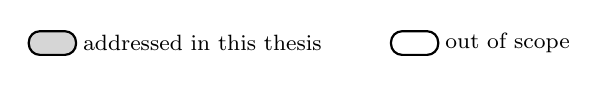
\begin{tikzpicture}[font=\footnotesize]
        \node[rectangle, draw, rounded corners, thick, fill=black!16,
            minimum width=0.6cm, minimum height=0.3cm] (in) at (0,0) {};
        \node[anchor=west, inner sep=2pt] at (in.east) {addressed in this thesis};
        \node[rectangle, draw, rounded corners, thick,
            minimum width=0.6cm, minimum height=0.3cm] (out) at (4.6,0) {};
        \node[anchor=west, inner sep=2pt] at (out.east) {out of scope};
    \end{tikzpicture}
\end{center}

    \begin{block}{Scope and overlap}
        \begin{itemize}
            \item State reachability is the common basis for Categories 1, 2a, and 2c
            \item Category 2b diagnosis needs graph analysis, Category 3 needs numeric fluents
            \item Categories overlap rather than partition, one problem may exhibit several types
        \end{itemize}
    \end{block}

    \sectioncite{Thesis \S4.1}
\end{frame}

%========================================================================
% Planning-native measures -- scenarios and normalization (Thesis \S4.3, \S4.4, \S4.6)
%========================================================================

\begin{frame}[noframenumbering]{Backup, reachable states and the horizon bound}
    \hypertarget{bk:reachability}{}
    \begin{block}{Reachable states}
        $S^0_{\text{reach}} = \{I\}$ \\[2pt]
        $S^{i+1}_{\text{reach}} = S^i_{\text{reach}} \cup \{\text{RESULT}(s, o) \mid s \in S^i_{\text{reach}},\ o \in O,\ \text{precond}(o) \subseteq s\}$
    \end{block}

    \begin{block}{Horizon bound}
        \begin{itemize}
            \item Ascending chain $S^0_{\text{reach}} \subseteq S^1_{\text{reach}} \subseteq \cdots$ converges at $h^* \leq 2^{|P|}$, each step only adds states
            \item $h^*$ is worst-case exponential, so the evaluation bounds it at $h = 20$
        \end{itemize}
    \end{block}

    \sectioncite{Thesis \S4.4.2}
\end{frame}

\begin{frame}[noframenumbering]{Backup, the isolated scenarios behind the running example}
    \hypertarget{bk:signatures}{}
    \begin{center}
        \scriptsize
        \begin{tabular}{l cc cc cc}
            \toprule
            Scenario         & \multicolumn{2}{c}{$\mathcal{I}_{\text{UR}}$} & \multicolumn{2}{c}{$\mathcal{I}_{\text{MX}}$} & \multicolumn{2}{c}{$\mathcal{I}_{\text{GS}}$}                           \\
            \cmidrule(lr){2-3}\cmidrule(lr){4-5}\cmidrule(lr){6-7}
                             & scope                                         & struct                                        & scope                                         & struct & scope & struct \\
            \midrule
            Locked Door      & 1                                             & 3                                             & 0                                             & 0      & 0     & 0      \\
            Bank Vault       & 1                                             & 7                                             & 0                                             & 0      & 0     & 0      \\
            Light Switch     & 0                                             & 0                                             & 2                                             & 1      & 0     & 0      \\
            Traffic Light    & 0                                             & 0                                             & 3                                             & 3      & 0     & 0      \\
            Trust and Travel & 0                                             & 0                                             & 2                                             & 1      & 2     & 1      \\
            Rival Alliances  & 0                                             & 0                                             & 2                                             & 1      & 2     & 2      \\
            \midrule
            Rover Mission    & 1                                             & 3                                             & 4                                             & 2      & 2     & 1      \\
            \bottomrule
        \end{tabular}
    \end{center}

    \begin{block}{The Rover Mission composes three canonical patterns}
        Drill chain $=$ Locked Door, dish toggle $=$ Light Switch, orbit chain $=$ Trust and Travel. The per-measure counts add to $(1, 3, 4, 2, 2, 1)$.
    \end{block}

    \sectioncite{Thesis \S4.3.4, \S4.4}
\end{frame}

\begin{frame}[noframenumbering]{Backup, absolute counts instead of normalized measures}
    \hypertarget{bk:normalization}{}
    \begin{exampleblock}{Relative measures exist [Besnard and Grant, 2020]}
        Dividing by $|G|$, $|P|$, or the maximal conflict count would yield percentage-style scores comparable across problem sizes.
    \end{exampleblock}

    \begin{block}{Why the profiles stay absolute}
        \begin{itemize}
            \item Severity is not proportional to size, 2 conflicting goals among 100 may be easier to repair than a complete clique on 3
            \item Every denominator choice encodes an assumption about problem structure
            \item Profiles carry relative information, scope against structure within each measure
            \item Future work could calibrate normalization against the IPC benchmark distribution
        \end{itemize}
    \end{block}

    \sectioncite{Thesis \S4.6.2}
\end{frame}

%========================================================================
% Postulates and complexity (Thesis \S4.5)
%========================================================================

\begin{frame}[noframenumbering]{Backup, postulate choice and the combined measure}
    \hypertarget{bk:postulates}{}
    \begin{block}{Why these three postulates}
        \begin{itemize}
            \item Classical postulates assume formula structure, planning has goals, operators, and states
            \item Adding operators can resolve conflicts, so Monotonicity reverses sign
            \item Modified postulates and the multi-measure approach follow the ASP precedent [Ulbricht et al., 2016]
        \end{itemize}
    \end{block}

    \sectioncite{Thesis \S4.5.1, \S6.3.6, \S7.4}
\end{frame}

\begin{frame}[noframenumbering]{Backup, adding an operator can raise $\mathcal{I}_{\text{MX}}$ and $\mathcal{I}_{\text{GS}}$}
    \hypertarget{bk:op-mono-ce}{}
    \begin{exampleblock}{One construction breaks both, $P = \{a, g_1, g_2\}$, $I = \{a\}$, $G = \{g_1, g_2\}$}
        \footnotesize
        Start with $O = \{\,\textit{reach\_g1} = \langle \{a\}, \{g_1\}, \{a\}\rangle\,\}$, then add $\textit{reach\_g2} = \langle \{a\}, \{g_2\}, \{a\}\rangle$.\\[2pt]
        \centering
        \begin{tabular}{lcc}
            \toprule
                                      & before add & after add \\
            \midrule
            $\mathcal{I}_{\text{MX}}$ & $(0, 0)$   & $(2, 1)$  \\
            $\mathcal{I}_{\text{GS}}$ & $(0, 0)$   & $(2, 2)$  \\
            \bottomrule
        \end{tabular}
    \end{exampleblock}

    \begin{block}{Why the value rises, and why $\mathcal{I}_{\text{UR}}$ is immune}
        \footnotesize
        \begin{itemize}
            \item Before, $g_2$ is unreachable, so no mutex pair and no sequencing conflict can form
            \item The added operator makes $g_2$ reachable but deletes $a$, which nothing re-adds, so no reachable state holds both goals
            \item This operator-induced mutex, with neither order achievable, raises $\mathcal{I}$, while $\mathcal{I}_{\text{UR}}$ only falls as $S^h_{\text{reach}}$ grows
        \end{itemize}
    \end{block}

    \sectioncite{Thesis \S4.5.1}
\end{frame}

\begin{frame}[noframenumbering]{Backup, sequencing implies mutex}
    \hypertarget{bk:seq-implies-mx}{}
    \begin{exampleblock}{Proposition}
        For any $\Pi$ and horizon $h$, if $(g_1, g_2)$ is a sequencing conflict with $g_2$ achievable, then $\{g_1, g_2\}$ is a mutex pair at horizon $h$.
    \end{exampleblock}

    \begin{block}{Proof sketch and counterexample}
        \begin{itemize}
            \item Sequencing makes both achievable, yet no trace has $g_1$ at $\sigma_i$, $g_2$ at $\sigma_j$, $i \leq j$
            \item The $i = j$ case is the mutex condition, which with achievability is the mutex definition
            \item On the Rover the sequencing pair $(\text{in\_orbit}, \text{mapped})$ is also one of the two mutex pairs, as the proposition predicts
            \item Converse fails on the dish toggle, $\{\text{aimed\_earth}, \text{aimed\_probe}\}$ is mutex yet reversible, so neither order is a sequencing conflict
        \end{itemize}
    \end{block}

    \sectioncite{Thesis \S4.5.2}
\end{frame}

\begin{frame}[noframenumbering]{Backup, PSPACE-completeness proof sketch}
    \hypertarget{bk:pspace-proof}{}
    \begin{block}{Membership of $\text{UPPER}_{\mathcal{I}_{\text{UR}}}$ in PSPACE}
        \footnotesize
        \begin{itemize}
            \item Guess an operator trace from $I$ in polynomial space, accept when $g$ appears
            \item NPSPACE $=$ PSPACE by Savitch, iterating over $|G|$ goals stays polynomial
        \end{itemize}
    \end{block}

    \begin{block}{Hardness via reduction from PlanSat}
        \footnotesize
        From $\Pi = \langle P, O, I, G \rangle$, build $\Pi' = \langle P \cup \{g^*\},\ O \cup \{o^*\},\ I,\ \{g^*\} \rangle$ with $o^* = \langle G, \{g^*\}, \emptyset \rangle$. Then $g^*$ is reachable iff $\Pi$ has a plan, so $\text{UPPER}_{\mathcal{I}_{\text{UR}}}$ at $k = 0$ decides PlanSat.
    \end{block}

    \begin{block}{Extends to MX, GS, and the other problems}
        \footnotesize
        \begin{itemize}
            \item For $\mathcal{I}_{\text{MX}}$ and $\mathcal{I}_{\text{GS}}$ a similar reduction makes the only path to $g_2$ delete $g_1$, so the pair is mutex or sequenced iff $\Pi$ is unsolvable
            \item LOWER is the complement of UPPER, EXACT checks both bounds, VALUE binary-searches UPPER, all staying in PSPACE or FPSPACE
        \end{itemize}
    \end{block}

    \sectioncite{Thesis \S4.5.3}
\end{frame}

\begin{frame}[noframenumbering]{Backup, PSPACE flattens the propositional multi-tier landscape}
    \hypertarget{bk:pspace-compare}{}
    \begin{exampleblock}{Decision-problem complexity, planning versus propositional $\mathcal{I}_c$}
        \centering
        \footnotesize
        \begin{tabular}{lll}
            \toprule
            Problem & Planning measures & Propositional $\mathcal{I}_c$ [Thimm and Wallner, 2016] \\
            \midrule
            UPPER   & PSPACE-complete   & NP-complete                                             \\
            LOWER   & PSPACE-complete   & coNP-complete                                           \\
            EXACT   & PSPACE-complete   & $D^p$-complete                                          \\
            VALUE   & FPSPACE           & FP$^{\text{NP}[\log n]}$-complete                       \\
            \bottomrule
        \end{tabular}
    \end{exampleblock}

    \begin{block}{Why the tiers collapse}
        \footnotesize
        \begin{itemize}
            \item Propositionally the base problem is satisfiability, NP-complete, so the measures stack into tiers above it
            \item For planning the base is PlanSat, already PSPACE-complete, a far larger ceiling
            \item PSPACE $=$ co-PSPACE collapses UPPER, LOWER, and EXACT, VALUE follows by polynomially many calls, so the gaps between measures vanish
        \end{itemize}
    \end{block}

    \sectioncite{Thesis \S4.5.3}
\end{frame}

%========================================================================
% Implementation (Thesis \S5)
%========================================================================

\begin{frame}[noframenumbering]{Backup, ASP reasoning modes, brave and cautious}
    \hypertarget{bk:asp-reasoning}{}
    \begin{block}{Execution traces and reasoning modes}
        \begin{itemize}
            \item Each answer set of the encoding is one execution trace, a state sequence from $I$
            \item Brave reasoning unions the answer sets, an atom holds if some trace produces it
            \item Cautious reasoning intersects them, an atom holds only if every trace produces it [Eiter and Gottlob, 1995]
        \end{itemize}
    \end{block}

    \begin{exampleblock}{Brave and cautious over two traces}
        Trace 1 makes $\{a, b\}$ reachable, trace 2 makes $\{a, c\}$ reachable. \\[2pt]
        $\text{BRAVE} = \{a, b, c\}$ reachable by some trace, \quad $\text{CAUTIOUS} = \{a\}$ by every trace.
    \end{exampleblock}

    \sectioncite{Thesis \S2.4}
\end{frame}

\begin{frame}[noframenumbering]{Backup, why ASP over SAT and MaxSAT}
    \hypertarget{bk:asp-vs-sat}{}
    \begin{block}{Reasons in favor of ASP}
        \begin{itemize}
            \item Default negation supports non-monotonic reasoning, matching reversed Operator Monotonicity
            \item Brave reasoning unions answer-set traces in one solver call, no manual enumeration
            \item ASP outperforms basic SAT encodings for inconsistency measures [Kuhlmann et al., 2025]
        \end{itemize}
    \end{block}

    \begin{block}{Trade-off acknowledged}
        Specialized MaxSAT beats ASP on classical formula-counting measures [Niskanen et al., 2023], and remains a future-work direction for scalability on planning-native measures.
    \end{block}

    \sectioncite{Thesis \S5, \S7.4}
\end{frame}

\begin{frame}[noframenumbering,fragile]{Backup, state-space exploration encoding}
    \hypertarget{bk:asp-listing}{}
    \begin{lstlisting}[style=asp]
time(0..horizon).
holds(P, 0) :- init(P).
% Applicability, positive and negative preconditions
neg_precond_violated(O, T) :- neg_precond(O, P), holds(P, T).
applicable(O, T) :- operator(O), time(T), T < horizon,
    not neg_precond_violated(O, T), holds(P, T) : precond(O, P).
% One operator per step, each choice a distinct trace
{ apply(O, T) : applicable(O, T) } 1 :- time(T), T < horizon.
% State transition with frame axiom
deleted(P, T) :- apply(O, T), delete(O, P).
holds(P, T+1) :- apply(O, T), add(O, P).
holds(P, T+1) :- holds(P, T), not deleted(P, T), time(T), T < horizon.
    \end{lstlisting}
    The choice rule branches into one answer set per execution trace. The frame axiom carries propositions forward unless an operator deletes them.

    \sectioncite{Thesis \S5.3.2}
\end{frame}

\begin{frame}[noframenumbering]{Backup, 80 automated tests verify the pipeline}
    \hypertarget{bk:validation}{}
    \begin{exampleblock}{Test suite}
        \begin{itemize}
            \item 80 tests across 8 categories, full suite runs in under one second
            \item 11 test scenarios match expected profiles exactly
            \item Categories cover scenarios, hierarchy, library API, end-to-end PDDL
        \end{itemize}
    \end{exampleblock}

    \begin{block}{Sample expected vs computed matches}
        \centering
        \scriptsize
        \begin{tabular}{lll}
            \toprule
            Category          & Scenario              & Profile              \\
            \midrule
            P1 Unreachability & Locked Door           & $(1, 3, 0, 0, 0, 0)$ \\
            P2 Mutex          & Traffic Light         & $(0, 0, 3, 3, 0, 0)$ \\
            P3 Sequencing     & Rival Alliances       & $(0, 0, 2, 1, 2, 2)$ \\
            Edge case         & Empty Goals           & $(0, 0, 0, 0, 0, 0)$ \\
            Edge case         & Negative Precondition & $(1, 1, 0, 0, 0, 0)$ \\
            \bottomrule
        \end{tabular}
    \end{block}

    \sectioncite{Thesis \S5.6}
\end{frame}

%========================================================================
% Evaluation (Thesis \S6)
%========================================================================

\begin{frame}[noframenumbering]{Backup, 3unsat and the $k$-tuple blind spot}
    \hypertarget{bk:3unsat}{}
    \begin{exampleblock}{Pairwise coexistence with no triple-satisfying state}
        \[
            G = \{g_1, g_2, g_3\}, \qquad
            S_{\text{reach}} \supseteq \{\{g_1, g_2\}, \{g_2, g_3\}, \{g_1, g_3\}\}
        \]
        Every pair is reachable together, yet no state satisfies all three.
    \end{exampleblock}

    \begin{block}{Consequence for the measures}
        \begin{itemize}
            \item All goals individually reachable, so $\mathcal{I}_{\text{UR}}(\Pi) = (0, 0)$
            \item No mutex pair exists in $S_{\text{reach}}$, so $\mathcal{I}_{\text{MX}}(\Pi) = (0, 0)$
            \item No ordered sequencing failure either, so $\mathcal{I}_{\text{GS}}(\Pi) = (0, 0)$
            \item All 20 completed \textit{3unsat} instances confirm this at every tested horizon
            \item Future work extends to $k$-tuple analysis for $|G| \geq 3$ failures
        \end{itemize}
    \end{block}

    \sectioncite{Thesis \S6.3.6, \S7.4}
\end{frame}
